\subsection{Diagrama de Implantação}
\label{sec:titSecDiagDeploy}

O Diagrama de Implantação determina as necessidades de \textit{hardware} do sistema, as características físicas como servidores, estações, topologias e protocolos de comunicação \cite{guedes2018uml}, destacando todos as necessidades físicas no qual o sistema deverá ser executado. Também é mostrado como será a distribuição dos módulos do sistema nos momentos onde a aplicação estará sendo executada em diferentes servidores.

\begin{figure}[H]
    \centering
    \caption{Representação do Diagrama de Implantação}
    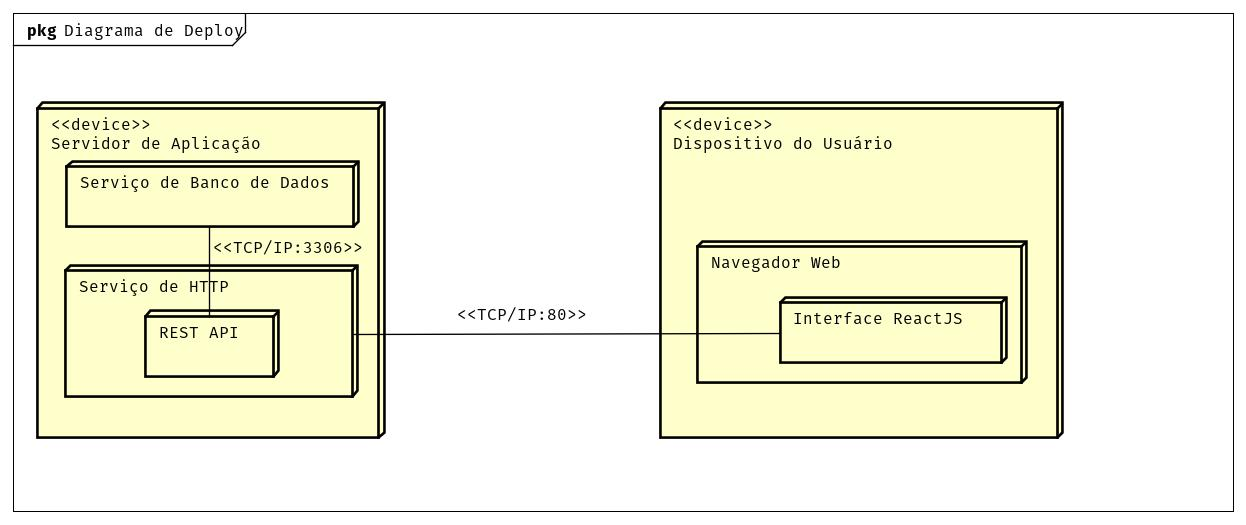
\includegraphics[width=13cm]{dados/figuras/diagramadeploy.jpg}
    \label{fig:diagramaDeploy}
    \fonte{Autoria própria}
\end{figure}

A \autoref{fig:diagramaDeploy} mostra a aplicação desse conceito no projeto. Nela é possível observar a distribuição do sistema em dois nós principais. O primeiro é o servidor de aplicação, que faz o encapsulamento do servidor Apache. Nesse mesmo servidor é possível observar a presença de um servidor MySQL, o qual será responsável por armazenar os dados do sistema e só receberá acessos locais.
O outro nó, representa o lado do cliente da aplicação, responsável pelas chamadas ao recursos contidos no servidor \textit{web} por meio de requisições Ajax, por meio do protocolo HTTP.
